\subsection{Dịch vụ xác thực (auth service - dùng Supabase)}


Hệ thống sử dụng Supabase để xử lý các nhóm chức năng chính bao gồm: xác thực và phân quyền, xác thực 2 yếu tố (MFA), quản lý dữ liệu người dùng và quản lý tệp tin (lưu trữ các file ảnh đại diện do người dùng tải lên tại bucket \texttt{avatars}).

Do mỗi lần người dùng đăng nhập lại, Supabase/Google sẽ ghi đè lại thông tin gốc từ tài khoản liên kết, bảng \texttt{profiles} được thiết kế riêng để lưu trữ và duy trì thông tin cập nhật mới nhất của người dùng.

Mô tả chi tiết các chức năng:

\subsubsection{I. Xác thực và Quản lý tài khoản}

Hệ thống sử dụng các API Auth của Supabase để xử lý toàn bộ luồng đăng nhập, đăng ký và bảo mật tài khoản:

\begin{itemize}
\item \textbf{Đăng nhập bằng Google}:
\begin{itemize}
\item Tạo URL và chuyển hướng người dùng đến trang ủy quyền của Google thông qua Supabase Auth Provider.
\item Endpoint sử dụng: \texttt{/auth/v1/authorize?provider=google\&redirect\_to=\{redirectUrl\}}
\end{itemize}

\item \textbf{Đăng nhập bằng Email và Mật khẩu}:
\begin{itemize}
\item Cho phép người dùng đăng nhập bằng tài khoản email. Trả về thông tin Access Token và Refresh Token nếu thành công.
\item Endpoint sử dụng: \texttt{/auth/v1/token?grant\_type=password}
\end{itemize}

\item \textbf{Đăng ký tài khoản mới}:
\begin{itemize}
\item Tạo tài khoản mới bằng Email và Mật khẩu, hỗ trợ gửi email xác nhận tài khoản thông qua đường dẫn chuyển hướng sau khi kích hoạt thành công (\texttt{redirect\_to}).
\item Endpoint sử dụng: \texttt{/auth/v1/signup}
\end{itemize}

\item \textbf{Khôi phục mật khẩu}:
\begin{itemize}
\item Gửi yêu cầu khôi phục mật khẩu tới email của người dùng. Hệ thống sẽ gửi một email chứa liên kết để xác thực và chuyển hướng người dùng về trang đổi mật khẩu.
\item Endpoint sử dụng: \texttt{/auth/v1/recover}
\end{itemize}

\item \textbf{Cập nhật mật khẩu mới}:
\begin{itemize}
\item Cho phép người dùng đổi mật khẩu mới sau khi đã đăng nhập (hoặc sau khi click vào liên kết khôi phục mật khẩu).
\item Endpoint sử dụng: \texttt{/auth/v1/user}
\end{itemize}

\item \textbf{Làm mới Access Token}:
\begin{itemize}
\item Sử dụng \texttt{refresh\_token} để lấy một \texttt{access\_token} mới khi token cũ hết hạn mà không bắt người dùng phải đăng nhập lại.
\item Endpoint sử dụng: \texttt{/auth/v1/token?grant\_type=refresh\_token}
\end{itemize}

\item \textbf{Đăng xuất}:
\begin{itemize}
\item Hủy phiên làm việc hiện tại của người dùng trên hệ thống Supabase Auth.
\item Endpoint sử dụng: \texttt{/auth/v1/logout}
\end{itemize}
\end{itemize}

\subsubsection{II. Xác thực 2 yếu tố (MFA)}

Hệ thống hỗ trợ phương thức xác thực hai yếu tố TOTP (Time-based One-Time Password - như Google Authenticator hay Authy) bằng các API nâng cao của Supabase:

\begin{itemize}
\item \textbf{Đăng ký thiết bị xác thực MFA mới}:
\begin{itemize}
\item Khởi tạo quá trình liên kết thiết bị xác thực mới. API trả về mã QR (\texttt{qr\_code}), mã bí mật (\texttt{secret}), và chuỗi URI để người dùng quét trên ứng dụng Authenticator.
\item Endpoint sử dụng: \texttt{/auth/v1/factors}
\end{itemize}

\item \textbf{Tạo thử thách xác thực}:
\begin{itemize}
\item Tạo một thử thách xác thực (challenge) dựa trên ID thiết bị MFA (\texttt{factorId}) để chuẩn bị so khớp với mã TOTP người dùng nhập.
\item Endpoint sử dụng: \texttt{/auth/v1/factors/\{factorId\}/challenge}
\end{itemize}

\item \textbf{Xác thực mã TOTP}:
\begin{itemize}
\item Kiểm tra mã TOTP gồm 6 chữ số người dùng nhập có khớp với thử thách hiện tại không. Nếu đúng, Supabase sẽ nâng cấp phiên làm việc của người dùng (tăng cấp bảo mật cho Access Token lên mức độ xác thực \texttt{aal2}).
\item Endpoint sử dụng: \texttt{/auth/v1/factors/\{factorId\}/verify}
\end{itemize}

\item \textbf{Lấy danh sách các yếu tố MFA}:
\begin{itemize}
\item Lấy thông tin tài khoản người dùng để lọc ra danh sách các thiết bị/yếu tố xác thực đã liên kết, phân loại thành: tất cả thiết bị (\texttt{all}) và các thiết bị đã kích hoạt thành công (\texttt{active}).
\item Endpoint sử dụng: \texttt{/auth/v1/user}
\end{itemize}

\item \textbf{Hủy liên kết/Xóa thiết bị MFA}:
\begin{itemize}
\item Xóa một thiết bị xác thực MFA khỏi tài khoản người dùng.
\item Endpoint sử dụng: \texttt{/auth/v1/factors/\{factorId\}}
\end{itemize}

\item \textbf{Cập nhật tên hiển thị của thiết bị MFA}:
\begin{itemize}
\item Đổi tên hiển thị (\texttt{friendly\_name}) của thiết bị xác thực (ví dụ: "Điện thoại cá nhân").
\item Endpoint sử dụng: \texttt{/auth/v1/factors/\{factorId\}}
\end{itemize}
\end{itemize}

\subsubsection{III. Quản lý Hồ sơ người dùng (Supabase Database - PostgREST API)}

Hệ thống sử dụng cơ chế RESTful API tự động sinh từ PostgreSQL của Supabase (PostgREST) để thực hiện các thao tác CRUD trên bảng cơ sở dữ liệu \texttt{profiles}:

\begin{itemize}
\item \textbf{Lấy thông tin hồ sơ}:
\begin{itemize}
\item Truy vấn thông tin chi tiết hồ sơ người dùng (như tên đầy đủ, ảnh đại diện) từ bảng \texttt{profiles} dựa vào \texttt{userId}.
\item Endpoint sử dụng: \texttt{/rest/v1/profiles?id=eq.\{userId\}}
\end{itemize}

\item \textbf{Cập nhật thông tin hồ sơ}:
\begin{itemize}
\item Cập nhật các trường thông tin hồ sơ như tên hiển thị (\texttt{full\_name}) hoặc đường dẫn ảnh đại diện (\texttt{avatar\_url}).
\item Endpoint sử dụng: \texttt{/rest/v1/profiles?id=eq.\{userId\}}
\end{itemize}
\end{itemize}

\subsubsection{IV. Quản lý Ảnh đại diện (Supabase Storage)}

Hệ thống sử dụng dịch vụ lưu trữ tệp (Storage) của Supabase để quản lý hình ảnh của người dùng:

\begin{itemize}
\item \textbf{Tải lên ảnh đại diện}:
\begin{itemize}
\item Tải tệp tin ảnh của người dùng lên thư mục \texttt{avatars} trên Supabase Storage. Tên tệp được sinh ngẫu nhiên kết hợp với \texttt{userId} để tránh trùng lặp.
\item Endpoint tải lên: \texttt{/storage/v1/object/avatars/\{fileName\}}
\item Đường dẫn công khai nhận về: \texttt{/storage/v1/object/public/avatars/\{fileName\}}
\end{itemize}
\end{itemize}

Thông tin payload của JWT từ Supabase:

\begin{figure}[H]
\centering
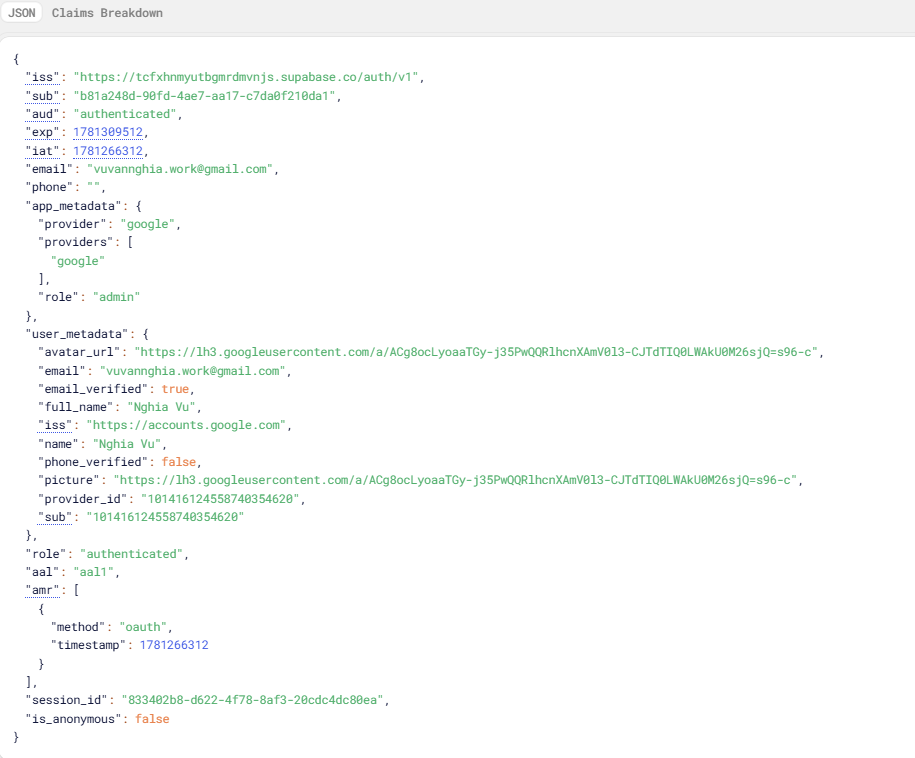
\includegraphics[width=0.85\textwidth]{pictures/auth-jwt-supabase.png}
\caption{Thông tin JWT Payload từ Supabase}
\label{fig:auth-jwt-supabase}
\end{figure}

Tham khảo tài liệu của Supabase tại:\\
\url{https://supabase.com/docs/guides/auth/auth-mfa/totp}

Trang tài liệu này hướng dẫn cách triển khai tính năng Xác thực Đa Yếu Tố (MFA) bằng ứng dụng Authenticator (TOTP) trong Supabase. Tính năng này hiện được cung cấp miễn phí và bật mặc định cho mọi dự án Supabase. Nội dung chính xoay quanh hai luồng hoạt động cơ bản:

\mbox{}\\
\textbf{Quy trình đăng ký yếu tố bảo mật (Enrollment Flow)}
\begin{enumerate}
\item Khởi tạo quá trình đăng ký.
\item Hệ thống sẽ trả về một mã QR và một chuỗi mã bí mật.
\item Người dùng sẽ dùng ứng dụng xác thực (như Google Authenticator) để quét mã QR này.
\item Chuẩn bị hệ thống để tiếp nhận mã xác minh, đồng thời trả về một challenge ID.
\item Đối chiếu mã 6 chữ số mà người dùng nhập vào từ ứng dụng xác thực.
\item Nếu mã hợp lệ, yếu tố bảo mật MFA này sẽ chính thức được kích hoạt cho tài khoản.
\end{enumerate}

\mbox{}\\
\textbf{Quy trình kiểm tra khi đăng nhập (Challenge Flow)}
\begin{enumerate}
\item Trích xuất danh sách các yếu tố MFA đã được người dùng đăng ký để lấy \texttt{factorId}.
\item Khi đã có \texttt{factorId}, ứng dụng tiếp tục gọi \texttt{challenge()} để mở phiên thử thách.
\item Dùng \texttt{verify()} cùng với mã OTP người dùng nhập vào để hoàn tất đăng nhập và nâng cấp phiên làm việc lên \texttt{aal2}.
\end{enumerate}

\begin{figure}[H]
\centering
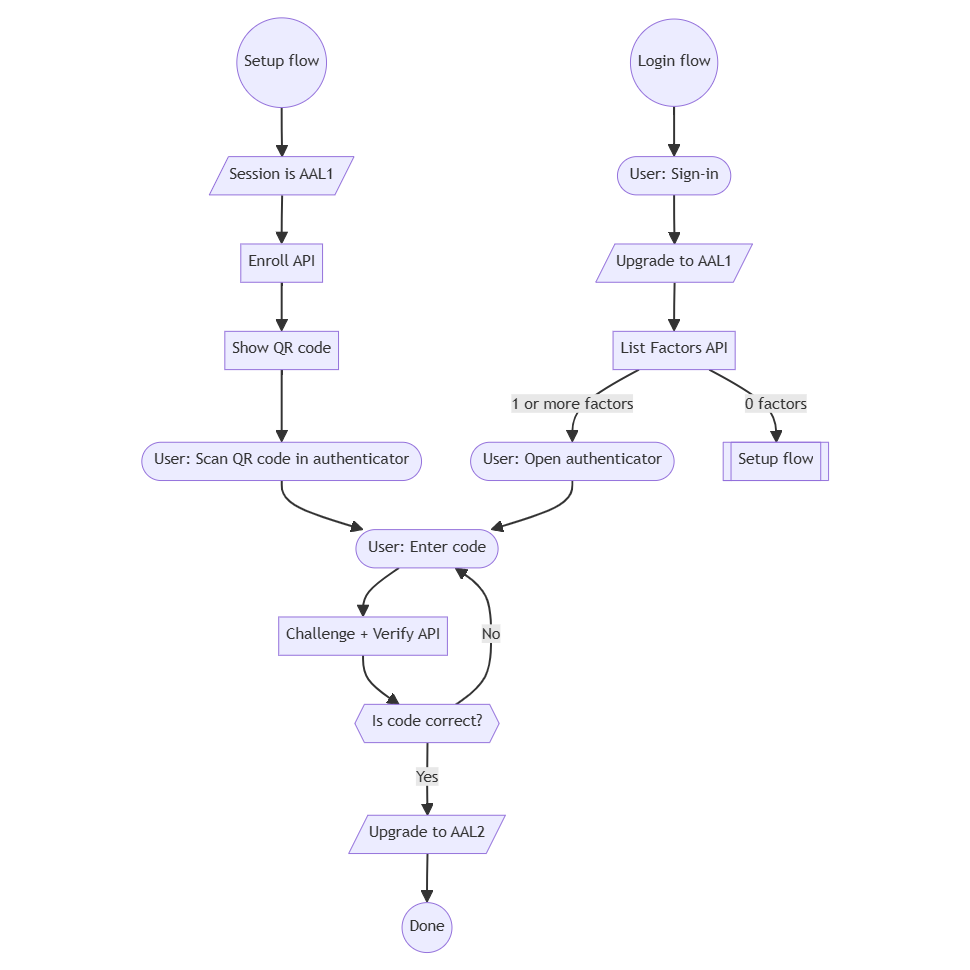
\includegraphics[width=0.7\textwidth]{pictures/auth-mfa-flow.excalidraw.png}
\caption{Sơ đồ luồng xử lý xác thực MFA}
\label{fig:auth-mfa-flow}
\end{figure}

Chi tiết về cấu hình Terraform dùng để quản lý hạ tầng Supabase:

\begin{figure}[H]
\centering
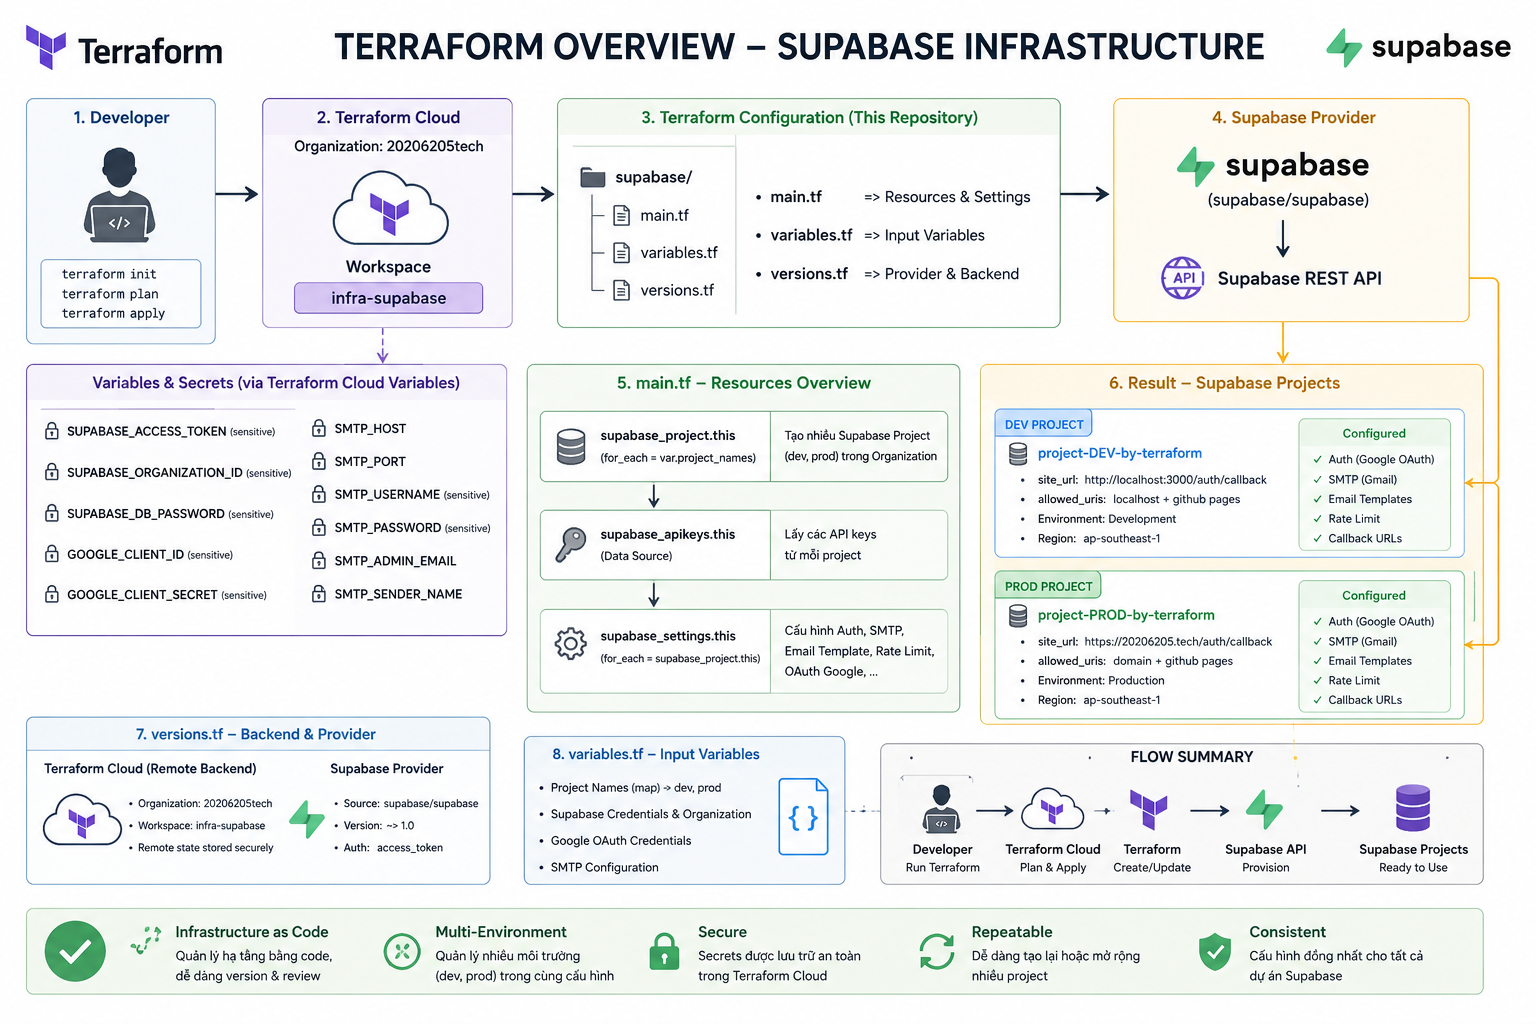
\includegraphics[width=0.85\textwidth]{pictures/auth-terraform-supabase-overview.png}
\caption{Tổng quan cấu hình Terraform quản lý hạ tầng Supabase}
\label{fig:auth-terraform-supabase-overview}
\end{figure}

Sử dụng Terraform Cloud với workspace \texttt{infra-supabase} để lưu trữ và quản lý trạng thái hạ tầng một cách tập trung.

Tự động tạo các dự án cho dev và prod dựa trên \texttt{project\_names}.

Cấu hình mã vùng (region) là \texttt{ap-southeast-1} tại Singapore để tối ưu tốc độ kết nối cho người dùng tại Việt Nam.

Bỏ qua sự thay đổi của mật khẩu nhằm tránh việc Terraform yêu cầu cập nhật hoặc thay đổi mật khẩu cơ sở dữ liệu sau mỗi lần chạy cấu hình.

Tích hợp đăng nhập qua Google OAuth (Client ID và Client Secret).

Thiết lập giới hạn gửi email (rate limit).

Cấu hình Hệ thống Email (SMTP) đang để mặc định là Gmail.

Ghi đè các mẫu email HTML cho "Xác nhận tài khoản" và "Đặt lại mật khẩu" để đồng nhất email thương hiệu tương tự như trong dịch vụ thanh toán.

\begin{figure}[H]
\centering
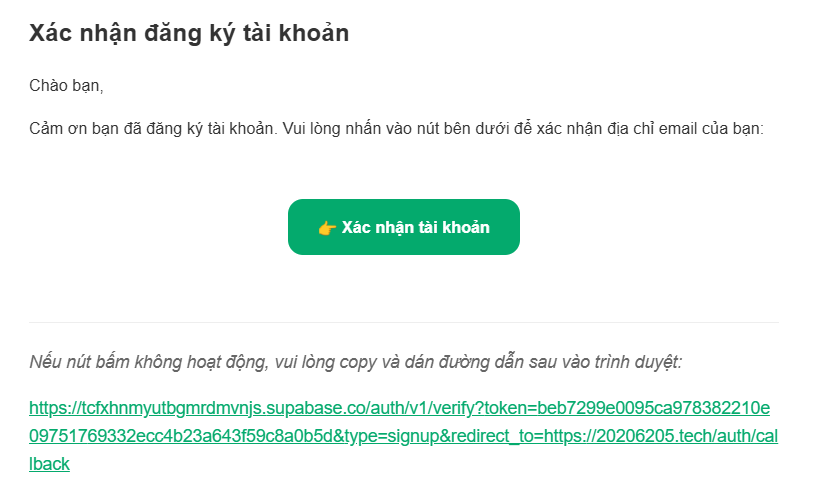
\includegraphics[width=0.85\textwidth]{pictures/auth-mail.png}
\caption{Mẫu email HTML được cấu hình}
\label{fig:auth-mail}
\end{figure}

\begin{figure}[H]
\centering
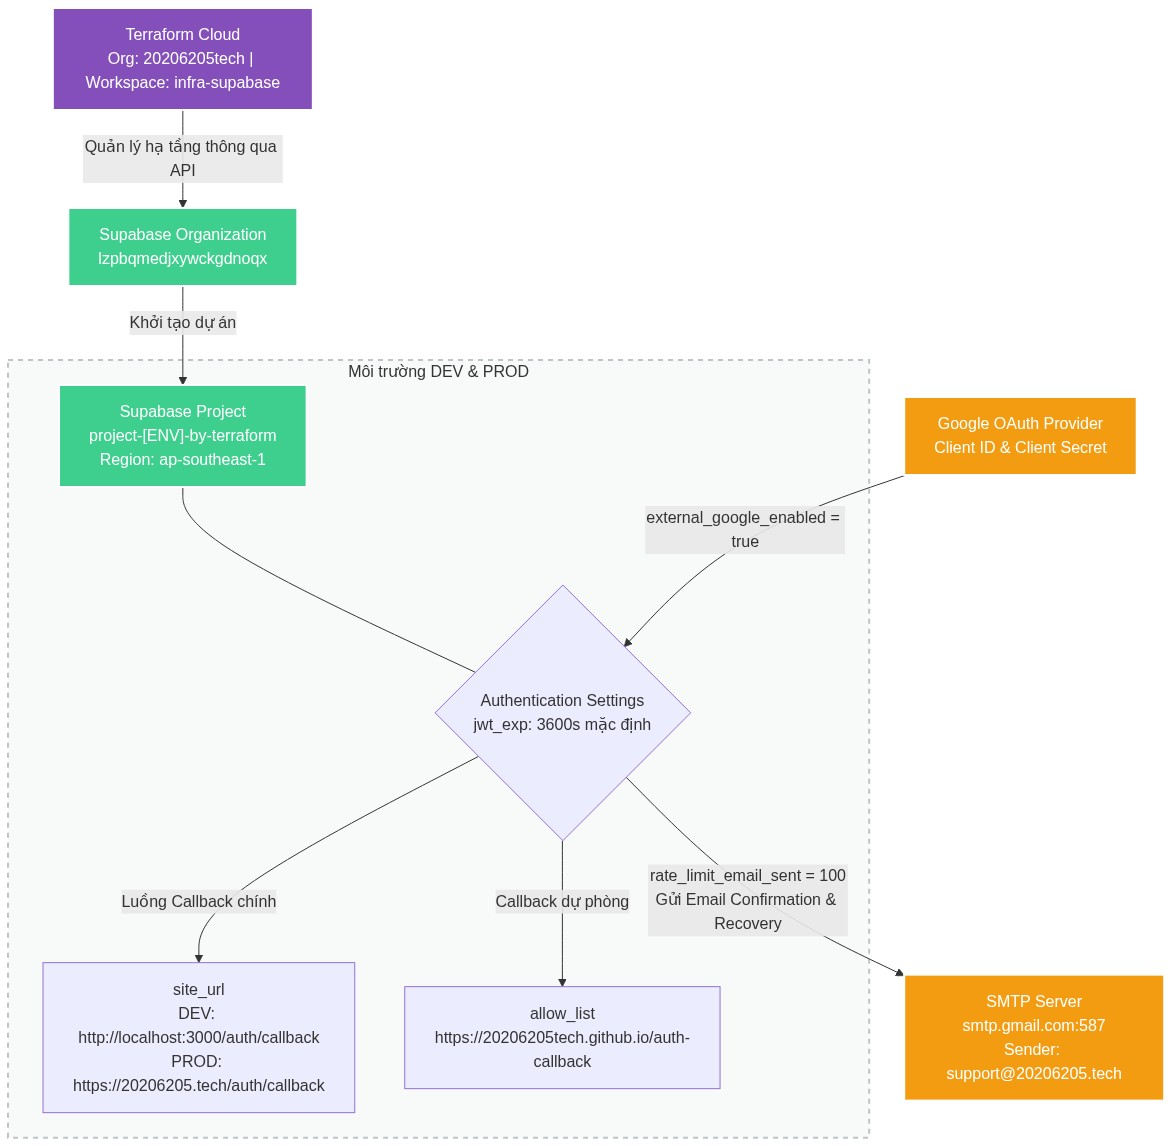
\includegraphics[width=0.85\textwidth]{pictures/auth-terraform-supabase-diagram.png}
\caption{Sơ đồ cấu hình Terraform cho Supabase}
\label{fig:auth-terraform-supabase-diagram}
\end{figure}

Chi tiết về cấu hình migration cơ sở dữ liệu Supabase:

Sử dụng Supabase CLI tạo dự án quản lý migration cơ sở dữ liệu bằng lệnh \texttt{npx supabase init}.

Trong thư mục migrations, các file SQL được thiết kế kết hợp với chính sách Bảo mật cấp hàng RLS (Row-Level Security):

\begin{itemize}
\item Tạo bảng \texttt{admin\_whitelist} lưu thông tin email của quản trị viên (ADMIN).
\item Tạo bucket \texttt{avatars} lưu thông tin file ảnh đại diện người dùng.
\item Tạo bảng \texttt{profiles} lưu thông tin của người dùng.
\item Tạo bucket \texttt{persona\_avatars} lưu thông tin file ảnh đại diện nhân vật.
\item Tạo bucket \texttt{persona\_audios} lưu thông tin file âm thanh lời chào nhân vật.
\end{itemize}

Kết quả bucket cấu hình trên Supabase:

\begin{figure}[H]
\centering
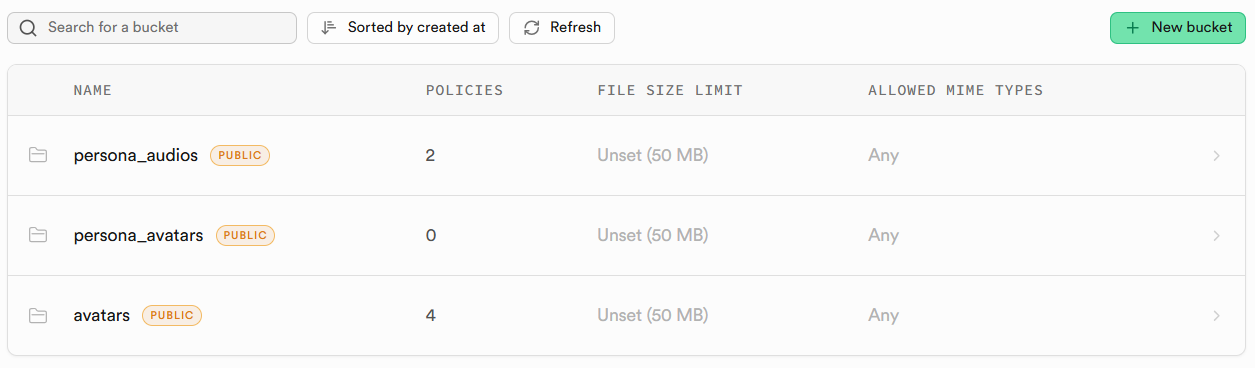
\includegraphics[width=0.85\textwidth]{pictures/auth-supabase-bucket.png}
\caption{Cấu hình các Storage Bucket trên Supabase}
\label{fig:auth-supabase-bucket}
\end{figure}

Kết quả cơ sở dữ liệu trên Supabase:

\begin{figure}[H]
\centering
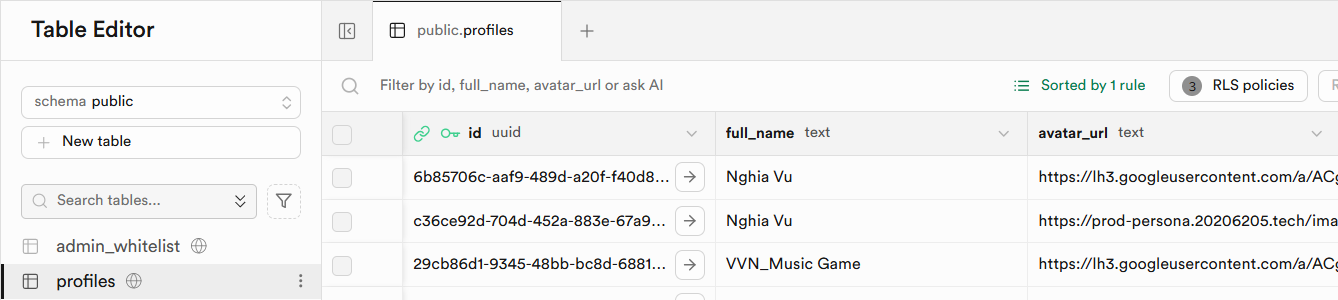
\includegraphics[width=0.85\textwidth]{pictures/auth-supabase-database.png}
\caption{Cấu hình bảng cơ sở dữ liệu trên Supabase}
\label{fig:auth-supabase-database}
\end{figure}

Để tối ưu hóa quá trình phát triển, các gói thư viện dùng chung (Shared Packages) đã được xây dựng để các dịch vụ khác dễ dàng tái sử dụng và quản lý:

Hiện tại trong dự án, có 2 gói thư viện dùng chung được xây dựng và đăng ký trên npm/PyPI là NestJS (\texttt{20206205tech-nestjs-auth}) và FastAPI trong Python (\texttt{20206205tech-python-auth}). Các thư viện này thực hiện các bước kiểm duyệt bảo mật tự động bao gồm:

\begin{figure}[H]
\centering
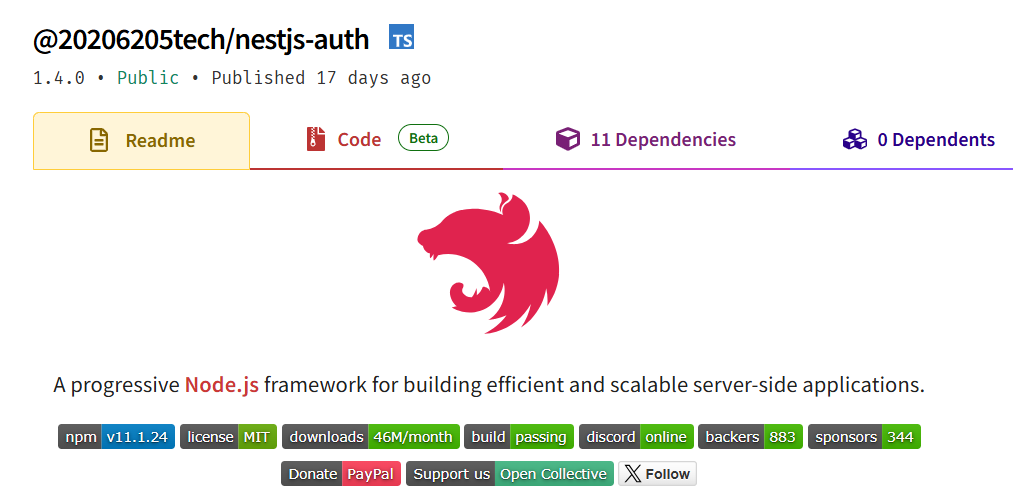
\includegraphics[width=0.85\textwidth]{pictures/nest-auth.png}
\caption{Quy trình kiểm tra bảo mật trong gói thư viện dùng chung}
\label{fig:nest-auth}
\end{figure}

\begin{itemize}
\item Xác thực \texttt{Request-Id} được chuyển tiếp từ Kong API Gateway.
\item Xác thực mã bảo mật \texttt{Request-Kong-Secret} để đảm bảo request thực sự đi qua API Gateway.
\item Kiểm tra tính hợp lệ của chữ ký JWT của người dùng thông qua Supabase.
\item Xác thực trạng thái MFA (yêu cầu bắt buộc để nâng cao bảo mật dữ liệu).
\item Kiểm tra và phân quyền vai trò người dùng (ví dụ: yêu cầu vai trò quản trị viên ADMIN đối với các API quản lý).
\end{itemize}

\subsubsection{Cấu hình trong Kong API Gateway}

Tạo Service trong Kong trỏ về URL của dự án Supabase (\texttt{https://[PROJECT\_REF].supabase.co}).

Thiết lập Route: Tạo một Route liên kết với Service vừa tạo. Tham số \texttt{strip\_path=true} đảm bảo Kong sẽ xóa tiền tố khỏi URI trước khi chuyển tiếp request đến Supabase.

Dùng plugin \texttt{request-transformer} để tự động thêm \texttt{apikey} vào header trước khi gửi đến Supabase.
